\chapter{Ergänzungen zur Simulation von Gold-PVD}

Im Folgenden sollen ergänzend die in Abschnitt~\ref{goldpvd} vorgestellten Simulationen auf nanostrukturierten Substraten dargestellt werden.
Die beiden Substrate wurden mit \SI{1}{\nano\meter} breiten Lamellen sowie \SI{1x1}{\nano\meter} breiten Säulen, die in beiden Fällen eine Höhe von \SI{1}{\nano\meter} haben, präpariert (Abbildung~\ref{fig:goldnanostructures}), um die Stabilität von Parsivald bei der Relaxierung solcher Substrate zu prüfen.
Es wird aufgrund der hohen Mobilität von Gold-Atomen auf der Oberfläche eine Relaxierung hinsichtlich einer geringeren Oberfläche erwartet, die nach kurzer Zeit ununterscheidbar von einer glatten Oberfläche sein sollte.

Diese Glättung der Oberfläche ist in Abbildungen~\ref{fig:goldnanostructures-step3} und~\ref{fig:goldnanostructures-step9} klar zu erkennen.
Wie man besonders an der Relaxierung der Säulen zu erkennen ist, findet die Glättung nicht ausschließlich durch eine Beschichtung der Oberfläche statt, sondern wird durch Relaxierung der Säulen zu einer glätteren Oberfläche erreicht.
Zum Zeitpunkt der vollständigen Relaxierung liegt die Dicke der abgeschiedenen Gold-Schicht mit ungefähr \SI{0.7}{\nano\meter} unterhalb der ursprünglichen Höhe des Oberflächenprofiles.

\vspace{3em}

\begin{figure}[bh]
  \captionsetup[subfigure]{singlelinecheck=false}
  \def\subfigwidth{0.49\textwidth}

  \begin{subfigure}[t]{\subfigwidth}
    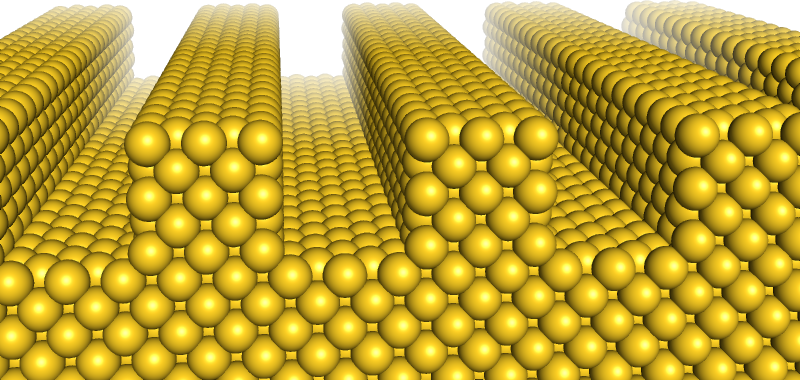
\includegraphics[width=\textwidth]{Au_fin_01}
    \subcaption{Gold-Lamellen, \SI{1}{\nano\meter} Breite}
    \label{fig:goldnanostructures-fins}
  \end{subfigure}
  \hfill
  \begin{subfigure}[t]{\subfigwidth}
    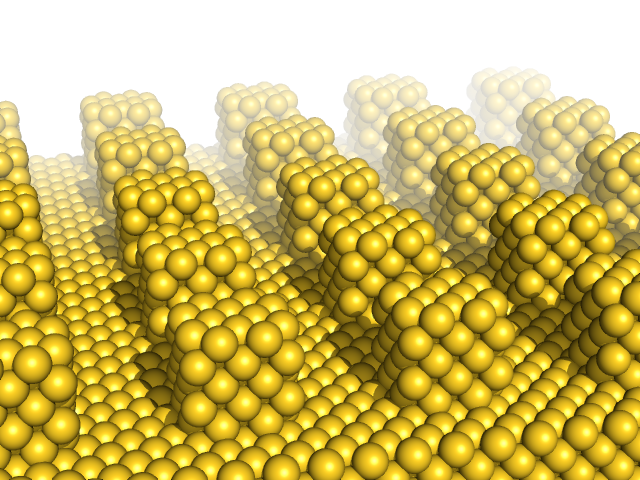
\includegraphics[width=\textwidth]{Au_pillars_1}
    \subcaption{Gold-Säulen, \SI{1x1}{\nano\meter} Breite}
    \label{fig:goldnanostructures-columns}
  \end{subfigure}

  \caption{Nanostrukturierte Substrate zur Simulation der Oberflächenrelaxierung mit Parsivald}
  \label{fig:goldnanostructures}

\end{figure}

\begin{figure}[!h]
  \captionsetup[subfigure]{singlelinecheck=false}
  \def\subfigwidth{0.49\textwidth}

  \begin{subfigure}[t]{\subfigwidth}
    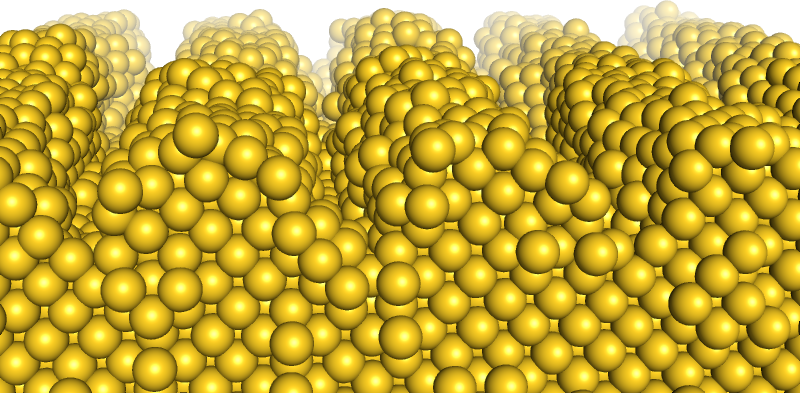
\includegraphics[width=\textwidth]{Au_fin_03}
    \subcaption{Substrat mit Gold-Lamellen}
    \label{fig:goldnanostructures-fins-step3}
  \end{subfigure}
  \hfill
  \begin{subfigure}[t]{\subfigwidth}
    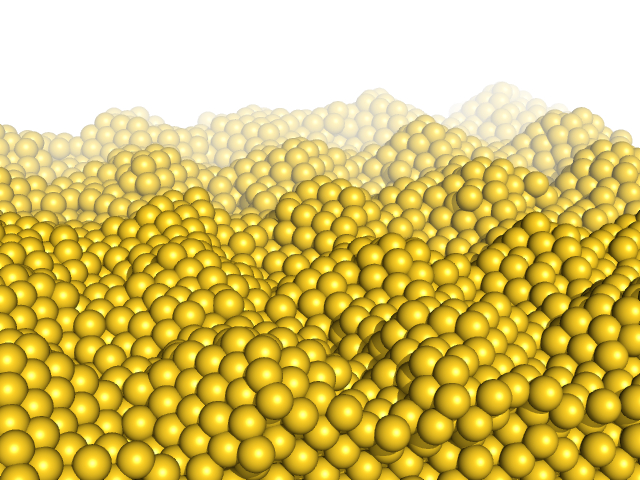
\includegraphics[width=\textwidth]{Au_pillars_3}
    \subcaption{Substrat mit Gold-Säulen}
    \label{fig:goldnanostructures-columns-step3}
  \end{subfigure}

  \caption{Oberfläche nach zwei Parsivald-Zyklen ($\approx \SI{2}{\angstrom}$ Schichtwachstum)}
  \label{fig:goldnanostructures-step3}

\end{figure}

\begin{figure}[!h]
  \captionsetup[subfigure]{singlelinecheck=false}
  \def\subfigwidth{0.49\textwidth}

  \begin{subfigure}[t]{\subfigwidth}
    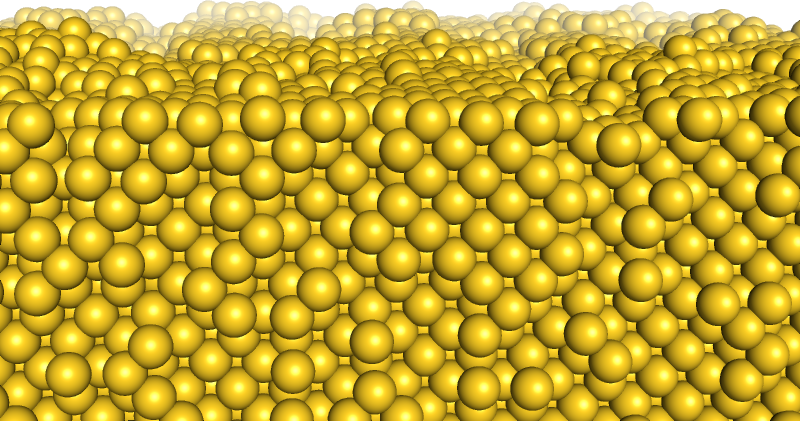
\includegraphics[width=\textwidth]{Au_fin_10}
    \subcaption{Substrat mit Gold-Lamellen}
    \label{fig:goldnanostructures-fins-step10}
  \end{subfigure}
  \hfill
  \begin{subfigure}[t]{\subfigwidth}
    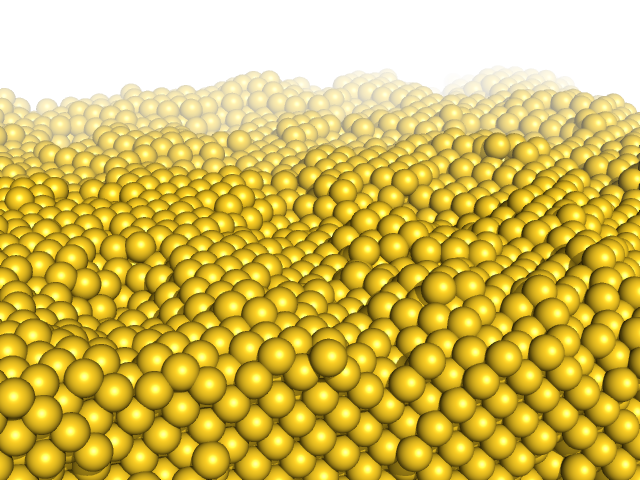
\includegraphics[width=\textwidth]{Au_pillars_8}
    \subcaption{Substrat mit Gold-Säulen}
    \label{fig:goldnanostructures-columns-step8}
  \end{subfigure}

  \caption{Oberfläche nach acht Parsivald-Zyklen ($\approx \SI{7}{\angstrom}$ Schichtwachstum)}
  \label{fig:goldnanostructures-step9}

\end{figure}
